\documentclass[10pt]{report}

\usepackage{talk}
\usepackage[export]{adjustbox}

\newcommand{\draw}[2]{#1^{(#2)}}
\newcommand{\displayfrac}[2]{{\displaystyle \frac{\displaystyle #1}{\displaystyle #2}}}
\newcommand{\simvar}[1]{#1^{\textrm{sim}}}
\newcommand{\simdraw}[2]{#1^{\textrm{sim}(#2)}}

\begin{document}
\sf%
\mbox{ }
\\[12pt]
\spc{\LARGE\bfseries \myemph{\slshape Bayesian Workflow:}}
\\[4pt]
\spc{\large\bfseries \myemph{Testing models and inferences}}
\\[24pt]
\noindent
\spc{\Large \myemph{Bob Carpenter}}
\\[4pt]
\spc{\large Center for Computational Mathematics}
\\[2pt]
\spc{\large Flatiron Institute}
\vfill
\noindent
\spc{\myemph{FWAM}, October 2024} \hfill

\includegraphics[width=1.5in]{img/flatiron-logo.png}
% \mypart{}{Motivation}

\sld{Textbook form of workflow}
\begin{enumerate}
    \item Set up a \myemph{full probability model}---a joint
      distribution for observables and unobservables consistent with
      knowledge about the scientific problem and data collection.
    \item \myemph{Condition on observed data}: calculate and interpret the
      \myemph{posterior distribution}.
    \item \myemph{Evaluate the fit and implications}: does it fit
      data, are conclusions reasonable, is it sensitive to
      assumptions?
    \item \myemph{Iterate}: If model fails evaluation, go back to (1).
      \begin{subitemize}
      \item For statisticians, last two steps were \myemph{revolutionary}.
      \end{subitemize}
    \end{enumerate}
      \vfill
      \spc {\footnotesize Gelman et al. 2013.  \textit{Bayesian Data
          Analysis, 3rd Edition}. Chapman \& Hall.}
    
\sld{Bayesian workflow involves}
\begin{subitemize}
  \item \myemph{designing experiments} and \myemph{collecting data},
  \item \myemph{designing / coding} probability models,
  \item evaluating \myemph{likelihoods} and \myemph{priors},
  \item \myemph{fitting} models to data,
  \item \myemph{validating} computation,
  \item addressing \myemph{computational issues},
  \item \myemph{evaluating} and \myemph{comparing} model fit and predictions,
  \item \myemph{modifying / improving} models, and
  \item \myemph{deploying} models predictively (prospective or retrospective).
    \vfill
  \end{subitemize}

\sld{Doesn't matter {\slshape how}\ you get inference}
\begin{itemize}
\item \myemph{Statistics} methods
\begin{subitemize}
\item Markov chain Monte Carlo
\item Sequential Monte Carlo
\item Variational inference (parametric)
\end{subitemize}
\item \myemph{Machine learning} methods
\begin{subitemize}
\item Variational inference (normalizing flow, diffusion densities)
\item Simulation-based inference (emulate likelihood with neural net)
\item Amortized inference (neural net mapping data to parameter estimates)
\end{subitemize}
\end{itemize}

\sld{A workflow chart}
\begin{center}
\vspace*{-6pt}
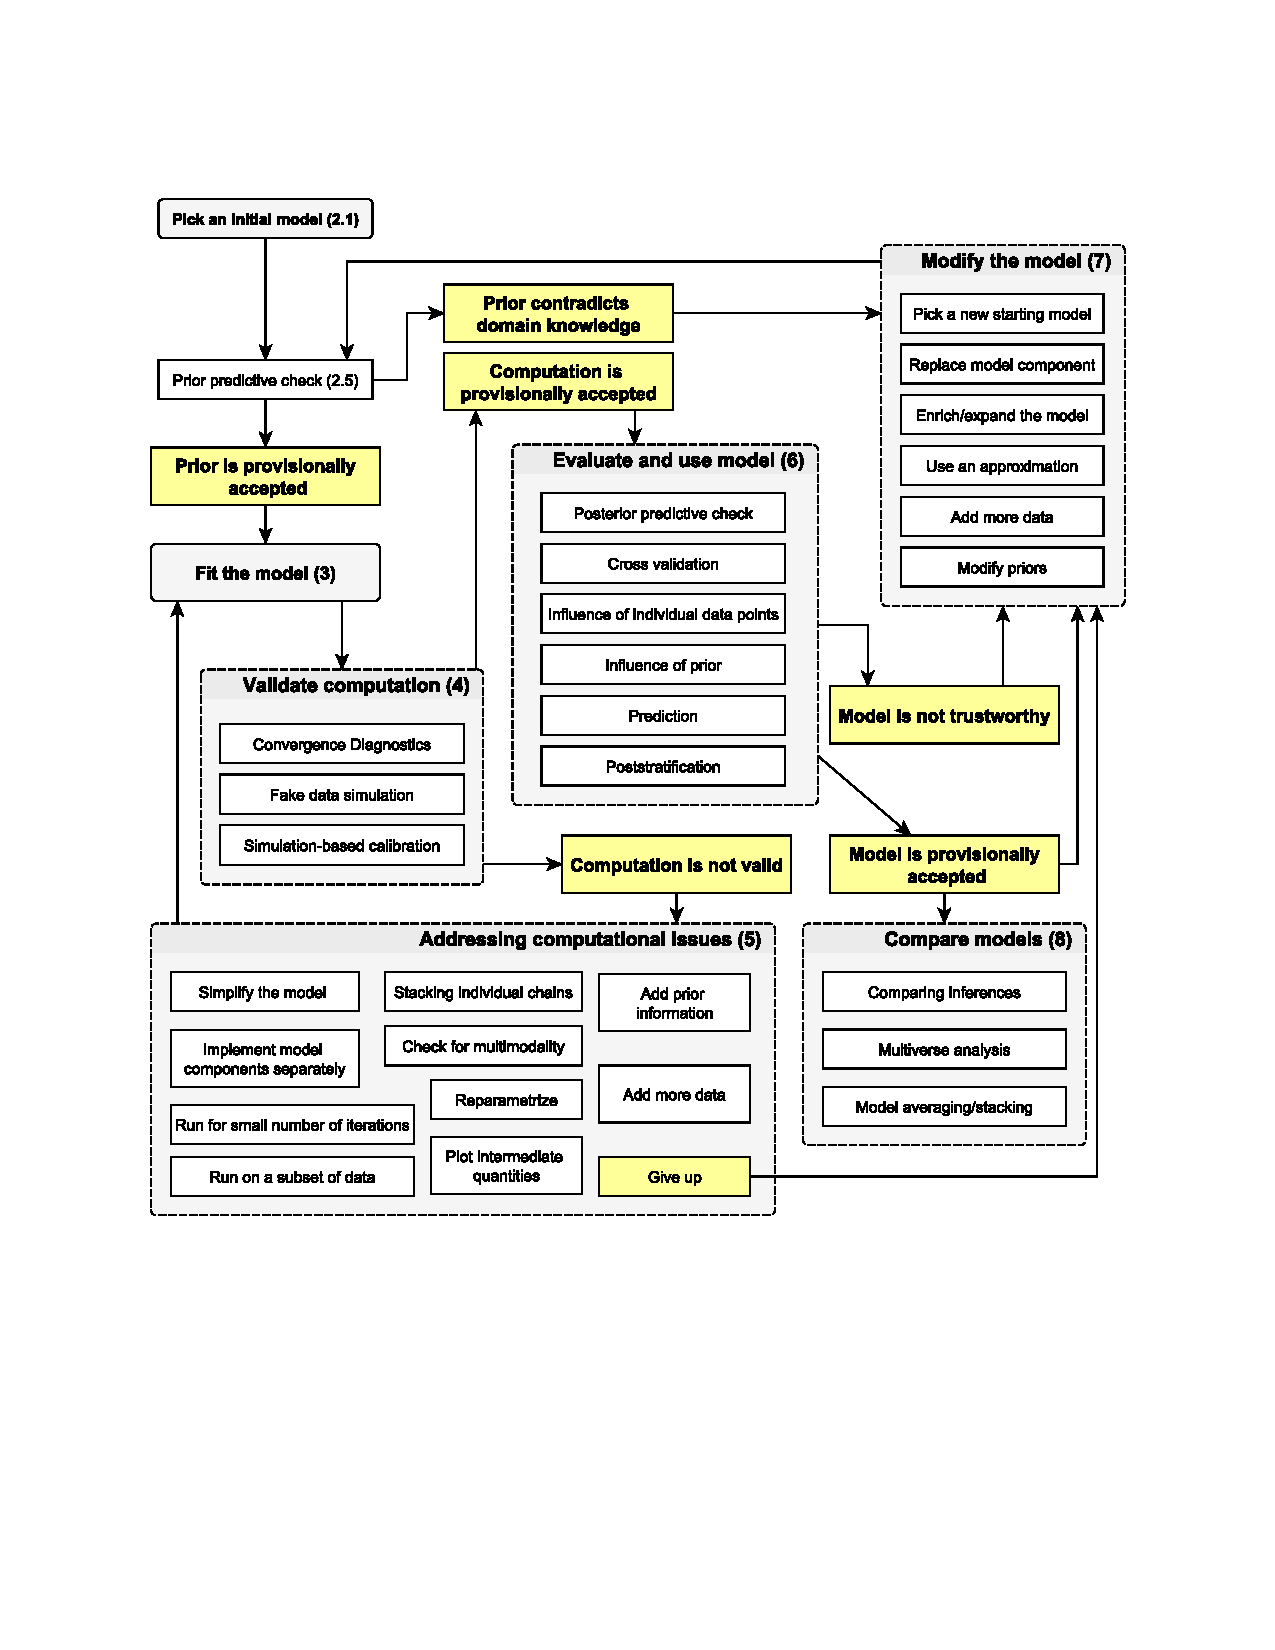
\includegraphics[height=0.85\textheight]{img/workflow-fig.pdf}
\\[-2pt]
\spc {\footnotesize Gelman et al. 2020.  Bayesian
        worflow. \textit{arXiv}.} \hfill \mbox{ }
\end{center}


\sld{Bayesian models}
\begin{itemize}
\item $y$ is \myemph{observed data}, $\theta$ are \myemph{unknown parameters}
\begin{subitemize}
\item suppress unmodeled predictors/features $x$
\end{subitemize}
\item \myemph{prior} distribution: $p(\theta)$
\item \myemph{sampling} distribution: $p(y \mid \theta)$
  \begin{subitemize}
    \item \myemph{likelihood} function: $\mathcal{L}(\theta) = p(y \mid \theta)$ for fixed $y$
  \end{subitemize}
\item \myemph{joint} distribution: $p(y, \theta) = p(y \mid \theta)\cdot p(\theta)$
\item \myemph{posterior} distribution:
  $$
  p(\theta \mid y)
  = \dfrac{p(y, \theta)}{p(y)}
  = \dfrac{p(y \mid \theta) \cdot p(\theta)}{\int p(y \mid \theta)
    \cdot p(\theta) \textrm{d}\theta}
  \propto p(y \mid \theta) \cdot p(\theta)
  $$
\end{itemize}

\sld{Prior and likelihood}
\begin{itemize}
\item The prior and likelihood can \myemph{only be understood
    together}
  \begin{subitemize}
  \item choosing both is \myemph{subjective}, but
  \item \myemph{likelihood more important}
    \item e.g., linear in log
      odds, compartment ode model, $\ldots$
  \end{subitemize}
\item The prior represents \myemph{what you already know}
  \begin{subitemize}
    \item often just \myemph{weakly informative} to \myemph{determine
        scale}
    \end{subitemize}
  \item \myemph{Sampling distribution} encodes \myemph{data
      generating process}
    \begin{subitemize}
    \item typically a scientific \myemph{forward model}
    \item coupled with a \myemph{noisy observation model}
    \end{subitemize}
  \end{itemize}

\sld{Estimating gravity \hfill {\normalsize (Galileo, Newton 17th c.)}}
\begin{itemize}
\item Roll balls down a ramp and \myemph{measure position vs.\ time $t$}.
\item Solve \myemph{Newton's differential equation} for expected position $\hat{y}(t)$ given (a) initial position,
  (b) slope of ramp, (c) \myemph{unknown gravitational constant} $G$, (d)
  measurement position.
\item Express \myemph{prior \slshape knowledge} as a distribution over plausible values
  of the gravitational constant: $G \sim \textrm{normal}(6.7, 0.2)$
\item Model the \myemph{measurement error} of your process
  probabilistically
  $y \sim \textrm{normal}(\hat{y}, \sigma)$.
\item Evaluate the \myemph{posterior} distribution to see what you
  \myemph{learned from data}: $p(G \mid y)$.
\end{itemize}

\sld{From the Galileo Museum}
\begin{center}
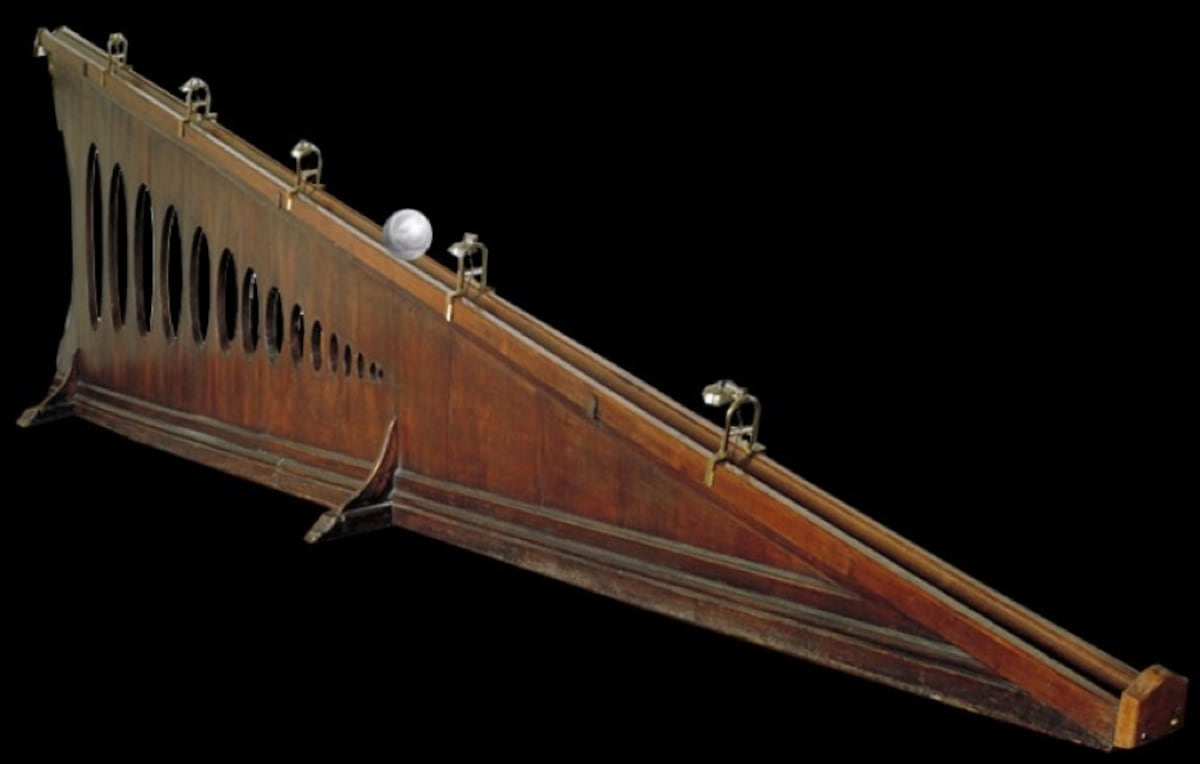
\includegraphics[width=0.8\textwidth]{img/galileo-plane.jpeg}
\end{center}

\sld{Simulate some data}
\begin{Verbatim}[fontsize=\small, xleftmargin=3ex]
import numpy as np

def sim(N, sigma, length, height):
    g = 9.81  # gravitational acceleration in m/s^2
    s = np.sqrt(length**2 + height**2)
    # solution for solid sphere moment of inertia
    t = np.sqrt((14 * s**2) / (5 * g * height))
    t_obs = np.random.lognormal(np.log(t), sigma, size=N)
    return {
        'length': length, 'height': height,
        'N': N, 't_obs': t_obs
      }
      
data = sim(N=100, sigma=0.1, length=5, height=2.5)
\end{Verbatim}

\sld{Code model in Stan}
\vspace*{-6pt}
\begin{stancode}
data {
  real<lower=0> length, height;  int<lower=0> N;  vector<lower=0>[N] t_obs;
}
transformed data {
  real<lower=0> s = hypot(length, height);
}
parameters {
  real<lower=0> g;      // gravity accel in m/s^2
  real<lower=0> sigma;  // measurement error scale
}
model {
  sigma ~ exponential(1);                 // weakly informative priors
  g ~ lognormal(log(10), 0.25);

  real log_t_true = 0.5 * (log(14) + 2 * log(s) - log(5) - log(g) - log(height));
  t_obs ~ lognormal(log_t_true, sigma);   // likelihood
}
\end{stancode}

\sld{Run posterior fit and plot}
\begin{stancode}
>>> import cmdstanpy as csp

>>> m = csp.CmdStanModel(stan_file='galileo.stan')
>>> draws = m.sample(data = data)
>>> draws.summary(sig_figs=2)
  
         Mean     MCSE  StdDev      5%     50%   95%  N_Eff  R_hat
lp__   98.000  0.02900  1.0000  95.000  98.000  98.0   1300    1.0
g       9.800  0.00310  0.1700   9.500   9.800  10.0   3000    1.0
sigma   0.089  0.00012  0.0064   0.079   0.088   0.1   2900    1.0
\end{stancode}
\begin{itemize}
\item Fit diagnostics good ($N_\text{eff}$ and $\widehat{R}$).
\item $g = 9.81, \sigma = 0.1$ recovered in
  central 90\% interval.
\item estimates $\widehat{g} \rightarrow 9.81$ and $\widehat{\sigma} \rightarrow 0.1$ as
  sample size $N \rightarrow \infty$
\end{itemize}



\sld{What makes inference Bayesian?}
\begin{itemize}
\item It's \myemph{not} the use of a prior.
\item It's \myemph{averaging over posterior uncertainty}.
\item Bayesian inference involves \myemph{posterior expectations},
  which are defined as posterior averages.
\end{itemize}

\sld{Parameter estimation}
\begin{itemize}
\item An \myemph{estimator} maps data $y$ to estimated parameter value.
\item \myemph{Bayesian parameter estimate} is posterior expectation
  $$
  \hat{\theta} = \mathbb{E}[\Theta \mid y] = \int_\Theta \theta \cdot
  p(\theta \mid y) \, \textrm{d}\theta
  $$
\item The posterior expectation is the estimate that \myemph{minimizes
    expected square error} (over random data sets $Y$),
  $$
  \hat{\theta} = \textrm{argmin}_\theta \ \mathbb{E}\!\left[\left( \strut\theta -
      \mathbb{E}\left[\theta \mid Y\right]\right)^2\right].
  $$
\item \myemph{Variance} estimates involve an expectation of $\theta^2$.
\end{itemize}
  
\sld{Event probability}
\begin{itemize}
\item An \myemph{event} $C$ is a subset of parameter space.
\item Bayesian \myemph{event probability estimate}
 $$
 \textrm{Pr}[C \mid y] = \mathbb{E}[\textrm{I}_C(\theta) \mid y]
 = \int_\Theta \textrm{I}_C(\theta) \cdot p(\theta \mid y) \, \textrm{d}\theta,
  $$
  where $\textrm{I}_C(\theta) = 1$ if $\theta \in C$ and $0$ otherwise.
\item Events \myemph{can be anything}, e.g., $\Pr[\Theta > 0.5 \mid y]$,
  \begin{subitemize}
  \item the event is $C = (0.5,1]$, where $\Theta$ is proportion
    of male live births and $y$ birth records
  \item Motivating example for Laplace, who derived $1 -
    10^{-42}$ from 50 years of Parisian birth records
    \end{subitemize}
\end{itemize}

\sld{Posterior predictive distribution}
\begin{itemize}
\item \myemph{Predicts new data} given observed data (and covariates).
\item \myemph{Posterior predictive distribution}
$$p(\tilde{y} \mid y) =
\mathbb{E}[p(\widetilde{y} \mid \Theta) \mid y]
= \int_\Theta p(\widetilde{y} \mid \theta) \cdot p(\theta \mid y) \, \textrm{d}\theta,
$$
where $\widetilde{y}$ is \myemph{new data}, $y$ is \myemph{observed
  data}, $\Theta$ parameters
\item \myemph{Averages} prediction of $\tilde{y}$ over uncertainty in
  $\Theta$
  given $y$
  \begin{subitemize}
\item $p(\widetilde{y} \mid \theta)$ is \myemph{sampling uncertainty}.
\item  $p(\theta \mid y)$ is \myemph{estimation uncertainty}.
  \end{subitemize}
\item Can \myemph{condition} everything on covariates
  \begin{subitemize}
    \item e.g., blood pressure,
      soil carbon concentration, etc.
  \end{subitemize}
\end{itemize}

\sld{Expectations via Monte Carlo}
\begin{itemize}
  \item calculate \myemph{asymptotically exact} expectations by averaging
\begin{eqnarray*}
  \mathbb{E}[f(\theta) \mid y]
  & = & \textstyle \int_{\Theta} f(\theta) \cdot p(\theta \mid y) \,
        \textrm{d}\theta
        \\[4pt]
  & = & \textstyle \lim_{M \rightarrow \infty} \frac{1}{M} \sum_{m = 1}^M
        f(\draw{\theta}{m})
        \\[4pt]
  & \approx & \textstyle \frac{1}{M} \sum_{m = 1}^M (\draw{\theta}{m}),
\end{eqnarray*}
\item MCMC \myemph{central limit theorem} says that if draws
\[
  \draw{\theta}{1}, \ldots, \draw{\theta}{M} \sim p(\theta \mid y)
\]
have \myemph{effective sample size} $M_{\textrm{eff}}$, then
\myemph{standard error} is
\[
\textrm{se}(\hat{\theta})
  = \displayfrac{\textrm{sd}[\theta \mid y]}
                {\sqrt{M_{\textrm{eff}}}} 
\]
\end{itemize}

\sld{PPLs}
\begin{itemize}
\item \myemph{Probabilistic programming languages} (PPLs)
\begin{subitemize}  
\item \myemph{code} Bayesian \myemph{joint densities} (up to
  constant), and
\item \myemph{sample} $\theta^{(n)} \sim p(\theta \mid y)$ from the
  posterior to compute expectations via Monte Carlo
\end{subitemize}
  \vfill
\item It turns out that
  \\
  we \myemph{need more than posterior sampling} for workflow.
\end{itemize}

\sld{Prior predictive checks}
\begin{itemize}
\item Prior predictive checks \myemph{simulate data} from the marginal
  \[
    \simvar{y} \sim p(y)
  \]
\item often by simulating from the \myemph{joint}, by generating from \myemph{prior} and \myemph{sampling} distributions
  \[
    \simvar{\theta} \sim p(\theta)
    \qquad
    \simvar{y} \sim p(y \mid \simvar{\theta})
  \]
\item Then \myemph{compare} simulated data $\simvar{y}$ to observed $y$
  \vfill
  {\footnotesize Gabry, Simpson, Vehtari, Betancourt,
    Gelman. 2019. Visualization in Bayesian workflow. \textit{JRSS A}.}
\end{itemize}

\sld{Prior predictive check}

\begin{itemize}
\item Evaluate whether \myemph{prior is sensible}
\begin{center}
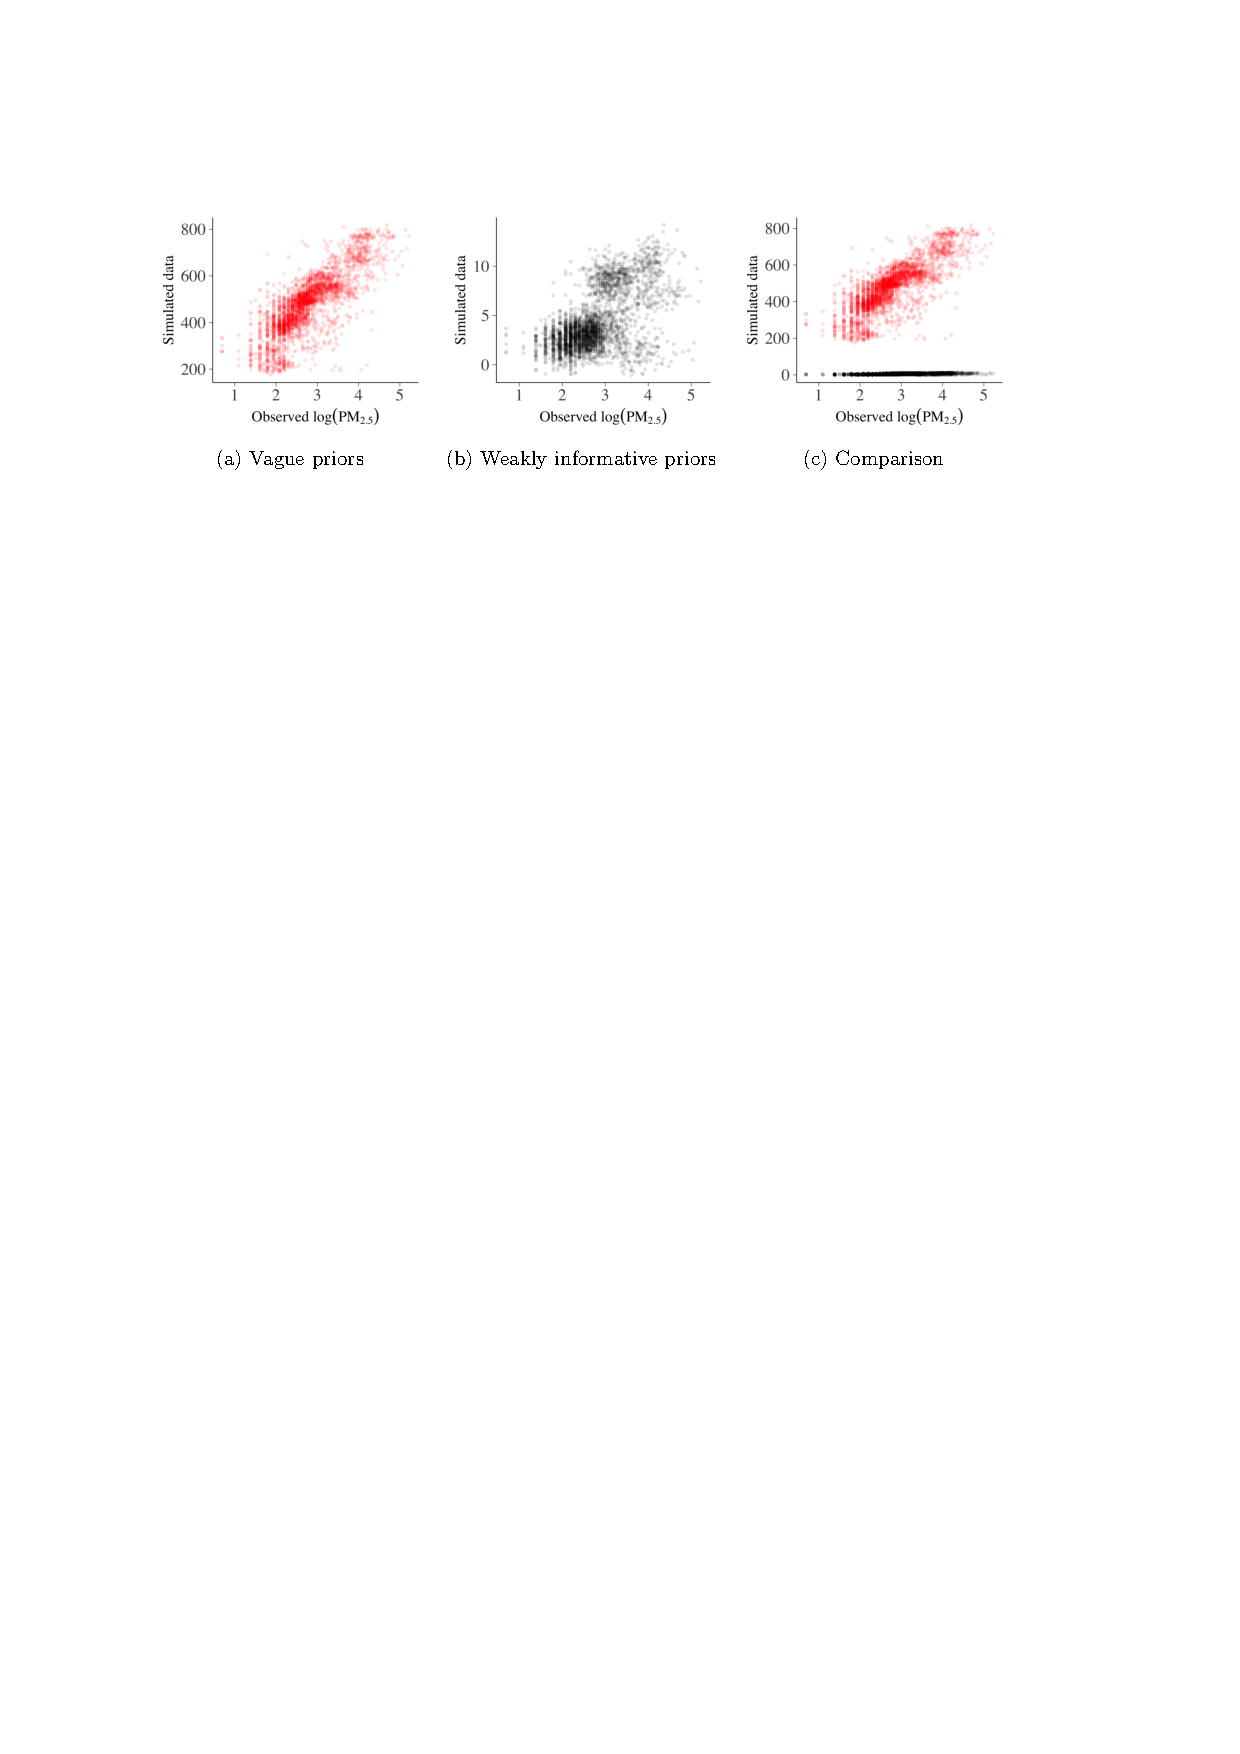
\includegraphics[width=0.75\textwidth]{img/prior-predictive-eg.pdf}
\end{center}
\vspace*{-10pt}
\item \myemph{particulate matter pollution} model with prior on
  $\log(\textrm{PM}_{2.5})$
\item \myemph{vague prior} generates values as dense as neutron star
\item \myemph{weakly informative} prior controls scale (subtle in \myemph{high dimensions})
\end{itemize}

\sld{Simulation-based Calibration}
\begin{itemize}
\item Evaluate whether \myemph{inference algorithm works}
  \begin{subitemize}
  \item Draw $\simvar{\theta} \sim p(\theta)$ from the prior
  \item Draw $\simvar{y} \sim p(y \mid \simvar{\theta})$ from the
    sampling distribution
  \item Draw $\draw{\theta}{1}, \ldots, \draw{\theta}{M} \sim p(\theta
    \mid \simvar{y})$ from algorithm to test
  \item Because $(\simvar{y}, \simvar{\theta}) \sim p(y, \theta)$ and
    $(\simvar{y}, \draw{\theta}{m}) \sim p(y, \theta)$,
    \\[4pt]
    $\simvar{\theta}$ and the $\draw{\theta}{m}$ \myemph{\slshape
      should}\ be \myemph{identically distributed} if sampler works
  \end{subitemize}
  \item Repeat and perform \myemph{statistical test}
    of uniformity of $\simvar{\theta}_d$ among $\draw{\theta}{m}_d$
    \vfill
    {\footnotesize Cook,  Gelman, Rubin.
      2006. Validation of software for Bayesian models using posterior
      quantiles. \textit{JCGS}.}
\end{itemize}

\sld{SBC diagnoses of inference failure}
\begin{itemize}
  \item 
    Posterior is \myemph{over-dispersed}: \hfill
    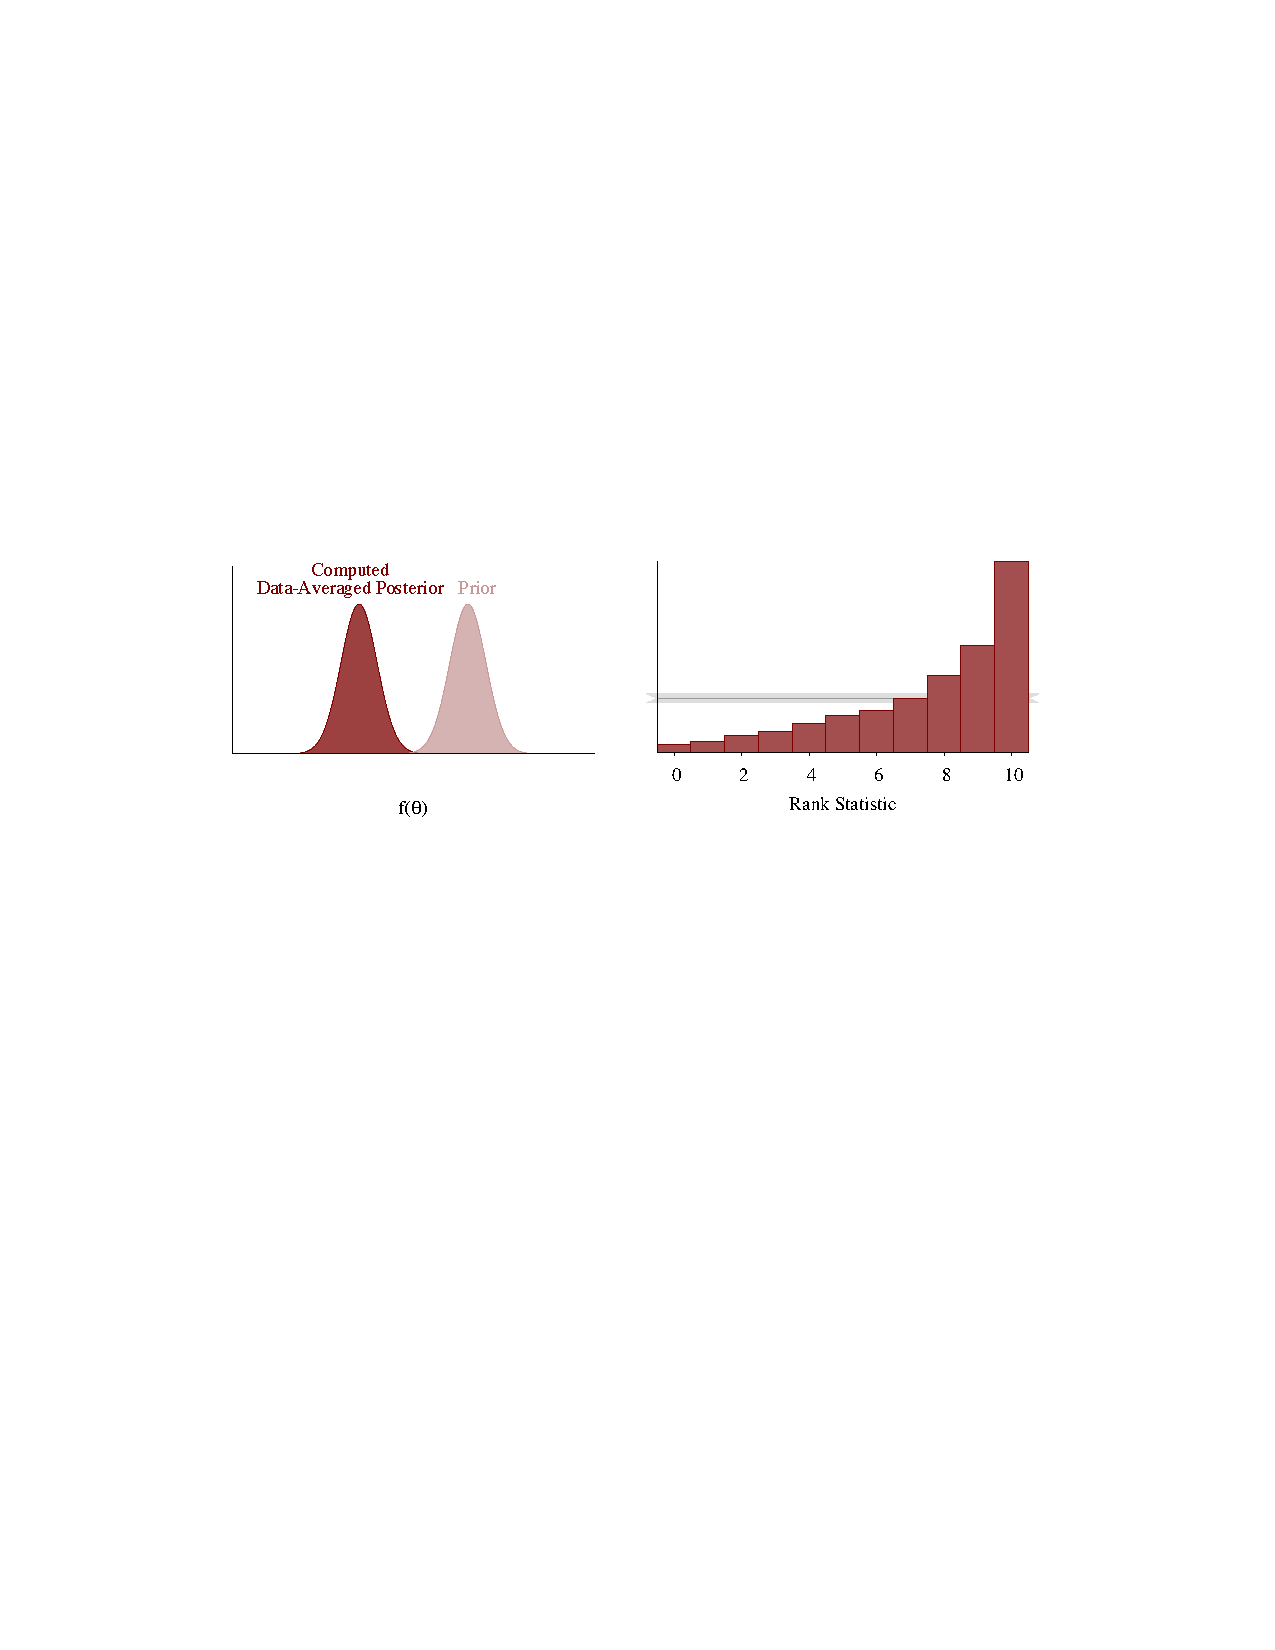
\includegraphics[valign=c,width=0.4\textwidth]{img/sbc-over.pdf}
  \item 
    Posterior is \myemph{under-dispersed}: \hfill
    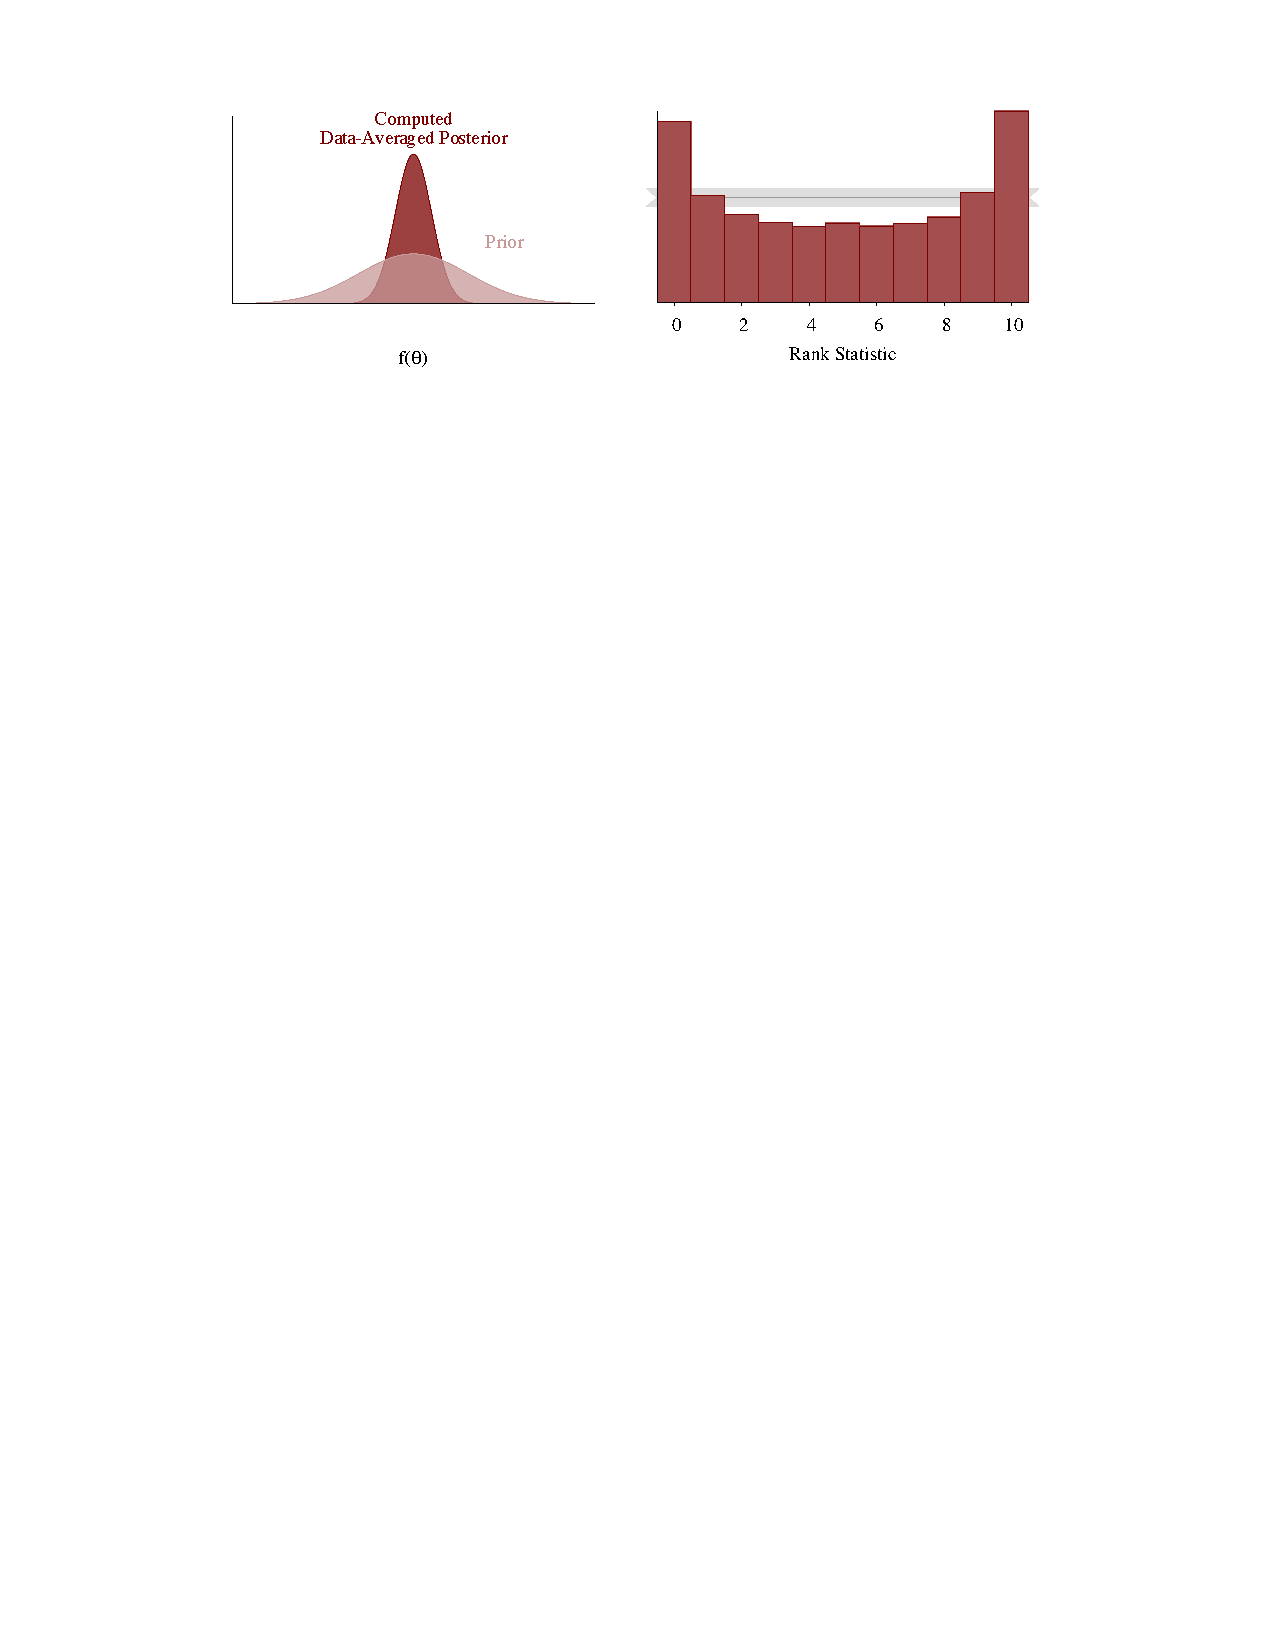
\includegraphics[valign=c,width=0.4\textwidth]{img/sbc-under.pdf}
  \item 
    Posterior is \myemph{biased}: \hfill
    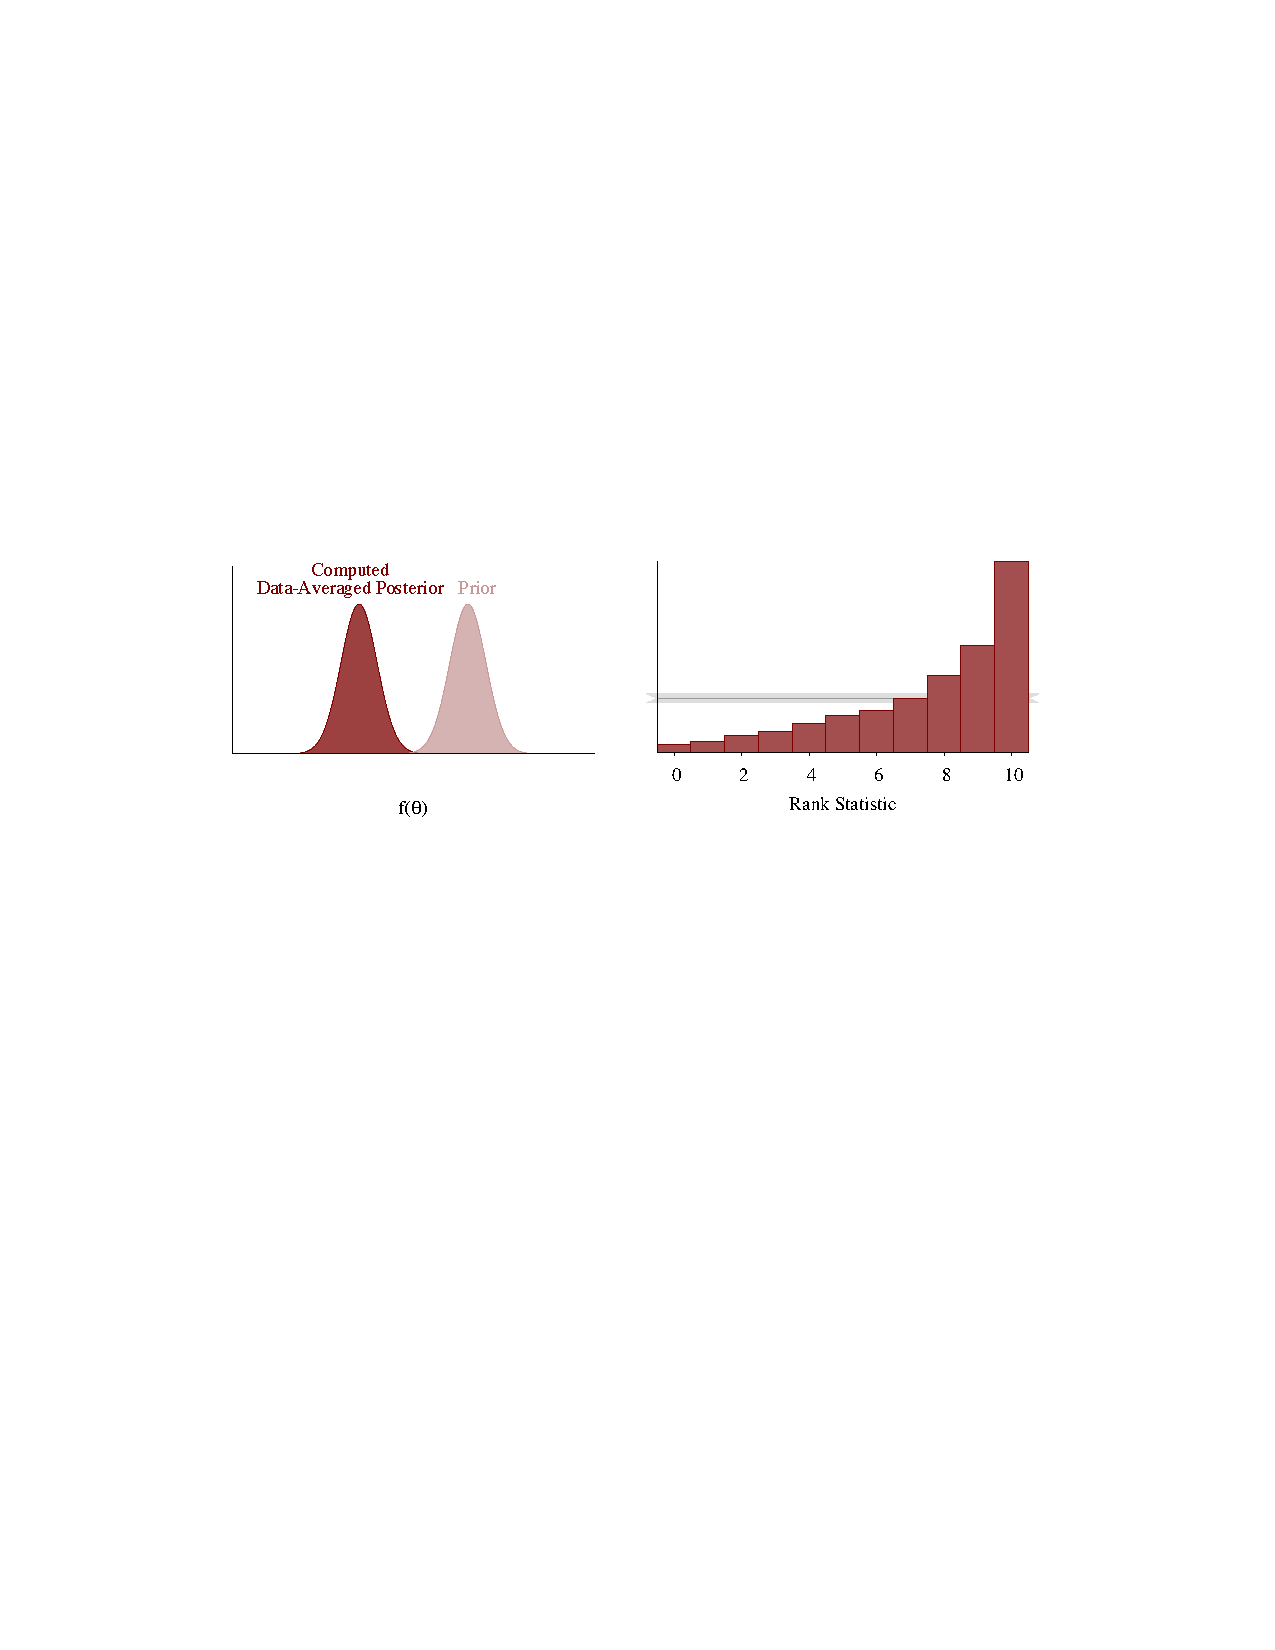
\includegraphics[valign=c,width=0.4\textwidth]{img/sbc-skew.pdf}
\end{itemize}



\sld{Posterior predictive checks}
\begin{itemize}
\item Evaluate whether \myemph{model is well-specified} for the data
\item Simulate new data from posterior for draws $m \in 1{:}M$,
  \begin{eqnarray*}
    \draw{\theta}{m} & \sim & p(\theta \mid y)
    \\
    \simdraw{y}{m} & \sim & p(y \mid \draw{\theta}{m})
  \end{eqnarray*}
\item Compare statistics $s(y)$ on observed data to those
  of posterior simulations $s(\simdraw{y}{m})$, e.g., mean, max, sd, quantiles, ranks,
\item Plot, or compute two-sided posterior $p$-values to automate,
  \[
    p\textrm{-value} = \min(\begin{array}[t]{l}
                              \textrm{Pr}[s(y) < s(\simvar{y})],
                              \\[4pt]
                              1 - \textrm{Pr}[s(y) < s(\simvar{y})] \ )
                              \end{array}
  \]
\end{itemize}

\sld{Posterior predictive example}
\begin{center}
\vspace*{-8pt}
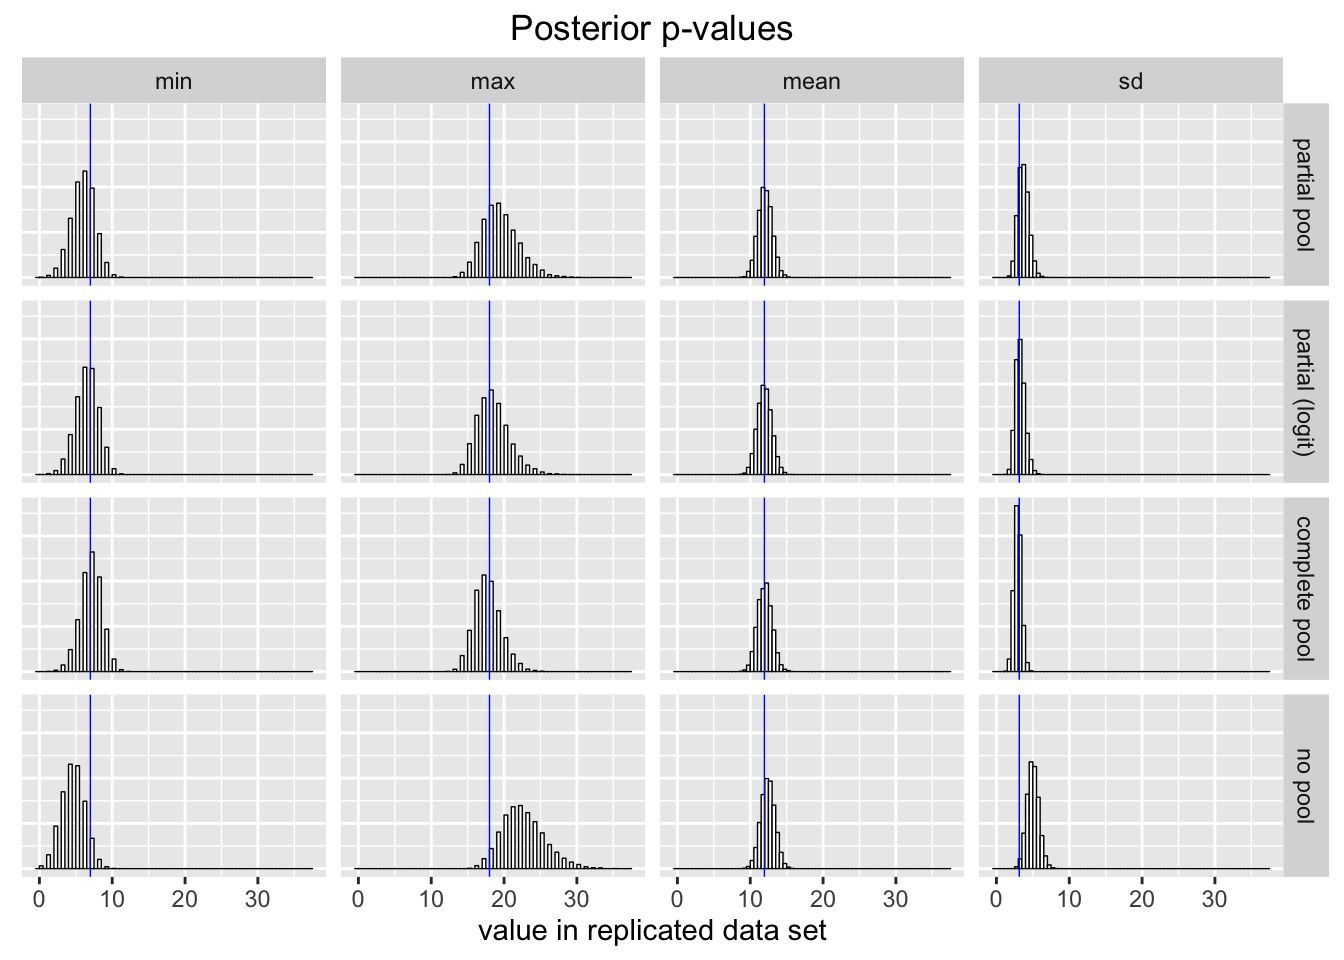
\includegraphics[width=0.525\textwidth]{img/ppc-binary-trials.png}
\vspace*{-6pt}
\end{center}
\begin{itemize}
\item model of repeated binary trials: \myemph{baseball batting
    average} by player
  \vspace*{-12pt}
  \begin{subitemize}
    \item vertical line is $s(y)$, histogram is $s(\simdraw{y}{m})$
    \item max() and sd() statistics ``reject'' the no-pooling model
  \end{subitemize}
\end{itemize}

\sld{Cross-validation}
\begin{itemize}
\item Evaluate whether \myemph{model is predictive} for new data.
\item divide data into train/test split (say $y$ and $\widetilde{y}$)
\item fit model on training set
\item evaluate predictive log density on test set,
  \begin{eqnarray*}
    \log p(\tilde{y} \mid y)
    & \approx & \log \frac{1}{M} \sum_{m=1}^M p(\tilde{y} \mid \simdraw{\theta}{m})
    \\[4pt]
    & = & \textrm{log-sum-exp}_{m=1}^M \, \log p(\tilde{y} \mid
          \simdraw{\theta}{m})
          - \log(M)
  \end{eqnarray*}
\end{itemize}

\sld{Sensitivity analysis}
\begin{itemize}
\item Evaluate whether \myemph{model is sensitive to prior}
\item \myemph{Empirical} sensitivity analysis
  \begin{subitemize}
    \item \myemph{vary priors} and measure how posterior changes
      (e.g., expectations)
    \end{subitemize}
\item \myemph{Derivative-based} sensitivity analysis
  \[
    \frac{\partial}{\partial c} \mathbb{E}[f(\theta) \mid y, c]
  \]
\end{itemize}  

\sld{Prior sensitivity example}

\spc{} \hspace{0.2in}{\footnotesize 0.01 \hspace{0.5in} 0.25 \hspace{0.5in} 0.5 \hspace{0.5in}
  0.75 \hspace{0.5in} 1.0}
\\[-8pt]
\begin{center}
\vspace*{-10pt}
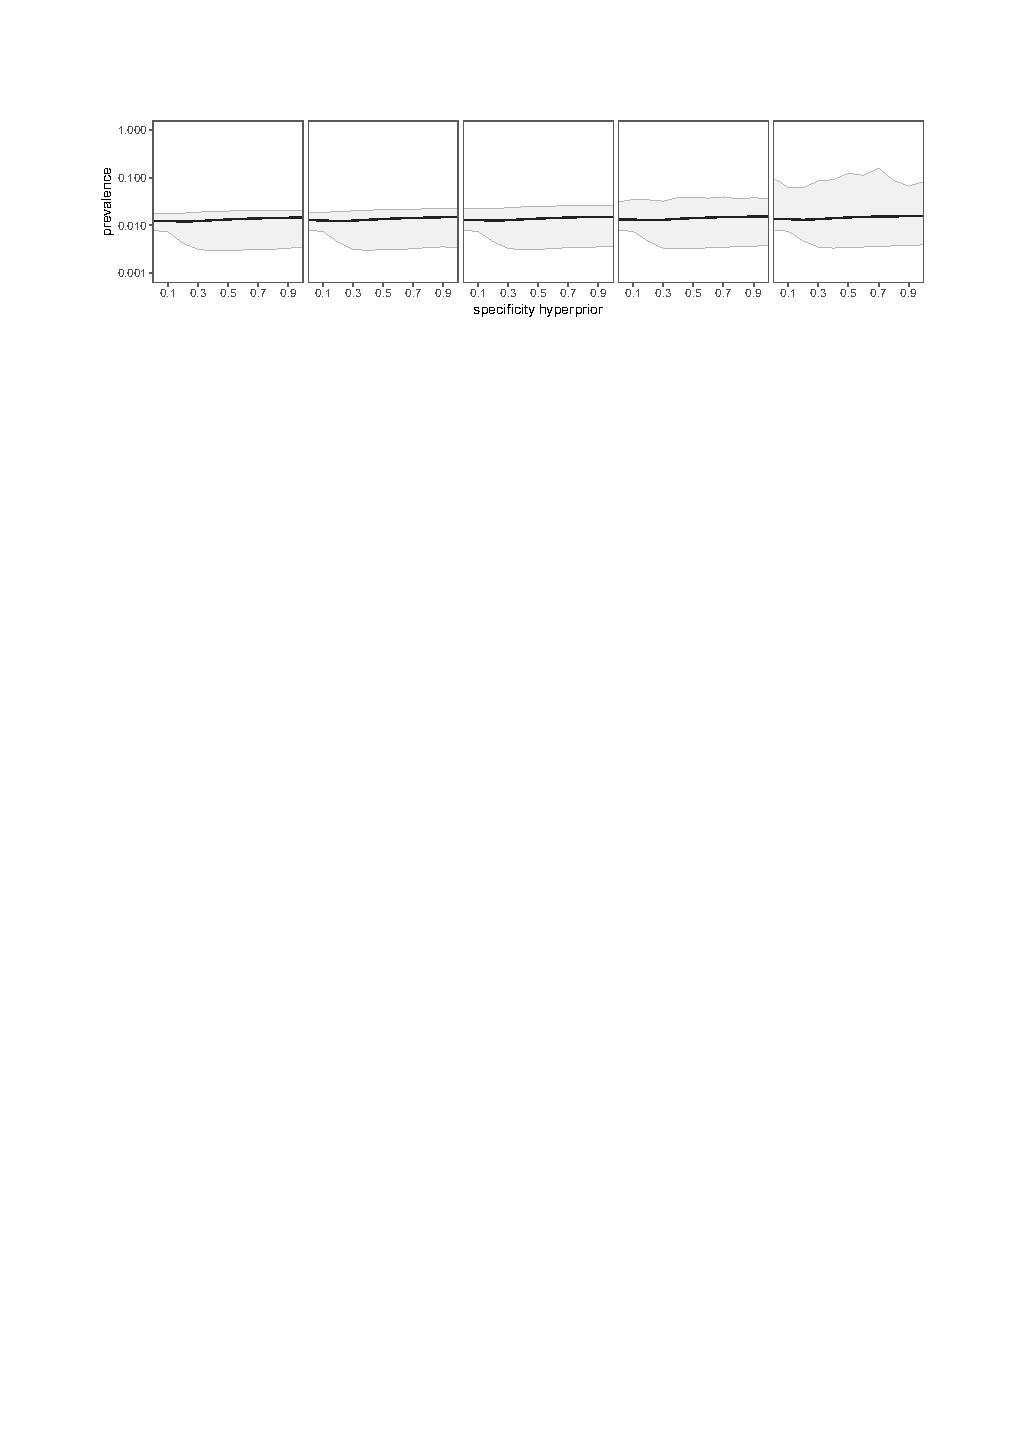
\includegraphics[width=0.9\textwidth]{img/covid-sensitivity.pdf}
\vspace*{-10pt}
\end{center}
\begin{itemize}
\item Estimated \myemph{Covid seroprevalence} 90\% interval ($y$ axis) vs.
  \begin{subitemize}
  \item \myemph{specificity hyperprior} scale ($x$-axis)
  \item \myemph{sensitivity hyperprior} scale (facets)
  \end{subitemize}
\vfill
{\footnotesize
Gelman, Carpenter. 2020. Bayesian analysis of tests with unknown
specificity and sensitivity. \textit{JRSS C}.}
\end{itemize}

\sld{Workflow goes beyond inference}
\begin{itemize}
\item \myemph{clamp/pin parameters} to fixed values?
  \begin{subitemize}
    \item Stan requires moving the variable from the parameter to the
      data block
  \end{subitemize}
\item working with \myemph{multiple (related) models}?
  \begin{subitemize}
  \item model comparison
  \item model reparameterization
  \item model averaging/mixing/stacking
  \end{subitemize}
\item \myemph{autogenerating} concurrent or GPU code?
  \begin{subitemize}
    \item Stan requires using parallel map functions in the program
  \end{subitemize}`
\end{itemize}

\sld{Naming and persistence is hard}
\begin{itemize}
\item How to \myemph{name and store multiple model variants}?
  \begin{subitemize}
    \item \texttt{uk-covid-icar}, \texttt{uk-covid-rw1}, \\
      \texttt{uk-covid-rw2}, \texttt{uk-covid-rw2-icar}, \\
      \texttt{uk-covid-rw2-bym2}, \texttt{uk-covid-rw2-bym2pc}, \\
      \texttt{uk-covid-rw2-bym2pc-no-socio},
      \textit{ad infinitum} $\ldots$
    \item plus multiple versions of the same model (over time)
  \end{subitemize}
\item How to \myemph{name and store output}?
\item How to work with \myemph{distributed teams}?
  \begin{subitemize}
  \item e.g., how to \myemph{share results} given that samples can be
    large?
  \item or that they run on clusters in pieces
  \end{subitemize}
\end{itemize}

\sld{Other workflow issues}
\begin{itemize}
\item Data may be tied up with \myemph{privacy} and/or \myemph{intellectual property}
  concerns
  \begin{subitemize}
  \item e.g., medical records, search logs, street views, etc.
  \end{subitemize}
\item End application may require \myemph{deployment in production}
  \begin{subitemize}
  \item e.g., bundle with Docker, or otherwise deploy
  \item \myemph{robustness} is a key issue
  \item \myemph{dynamically update} as new data comes in
  \end{subitemize}
  \vfill
  \item \myemph{What are we missing?}
\end{itemize}

\sld{References}
\begin{itemize}
\item \myemph{workflow paper}
  \begin{subitemize}
    \item Gelman, Vehtari, Simpson, Margossian, Carpenter, Yao, Kennedy,
    Gabry, Bürkner, Modrák. 2020. Bayesian workflow. \textit{arXiv}.
  \end{subitemize}
\item open-access \myemph{workflow book}
  \begin{subitemize}
  \item Above authors give or take. 2025(?) \textit{Bayesian Workflow}. Chapman \& Hall/CRC.
  \item GitHub repo: \\ {\small \url{https://github.com/jgabry/bayes-workflow-book}}
  \end{subitemize}
\end{itemize}
  

\end{document}

\vspace*{-6pt}
{\footnotesize 
\begin{verbatim}
\end{verbatim}
\vspace*{-8pt}}

\item \footnotesize Gelman, Vehtari, Simpson, Margossian, Carpenter, 
    Yao, Kennedy, Gabry, Bürkner, and Modrák. 2020. \myemph{Bayesian workflow}. 
    \textit{arXiv} 2011.01808.
  \item Book draft:
    \url{https://github.com/jgabry/bayes-workflow-book}

    \sld{Workflow's more than inference!}
\begin{center}
\vspace*{-6pt}
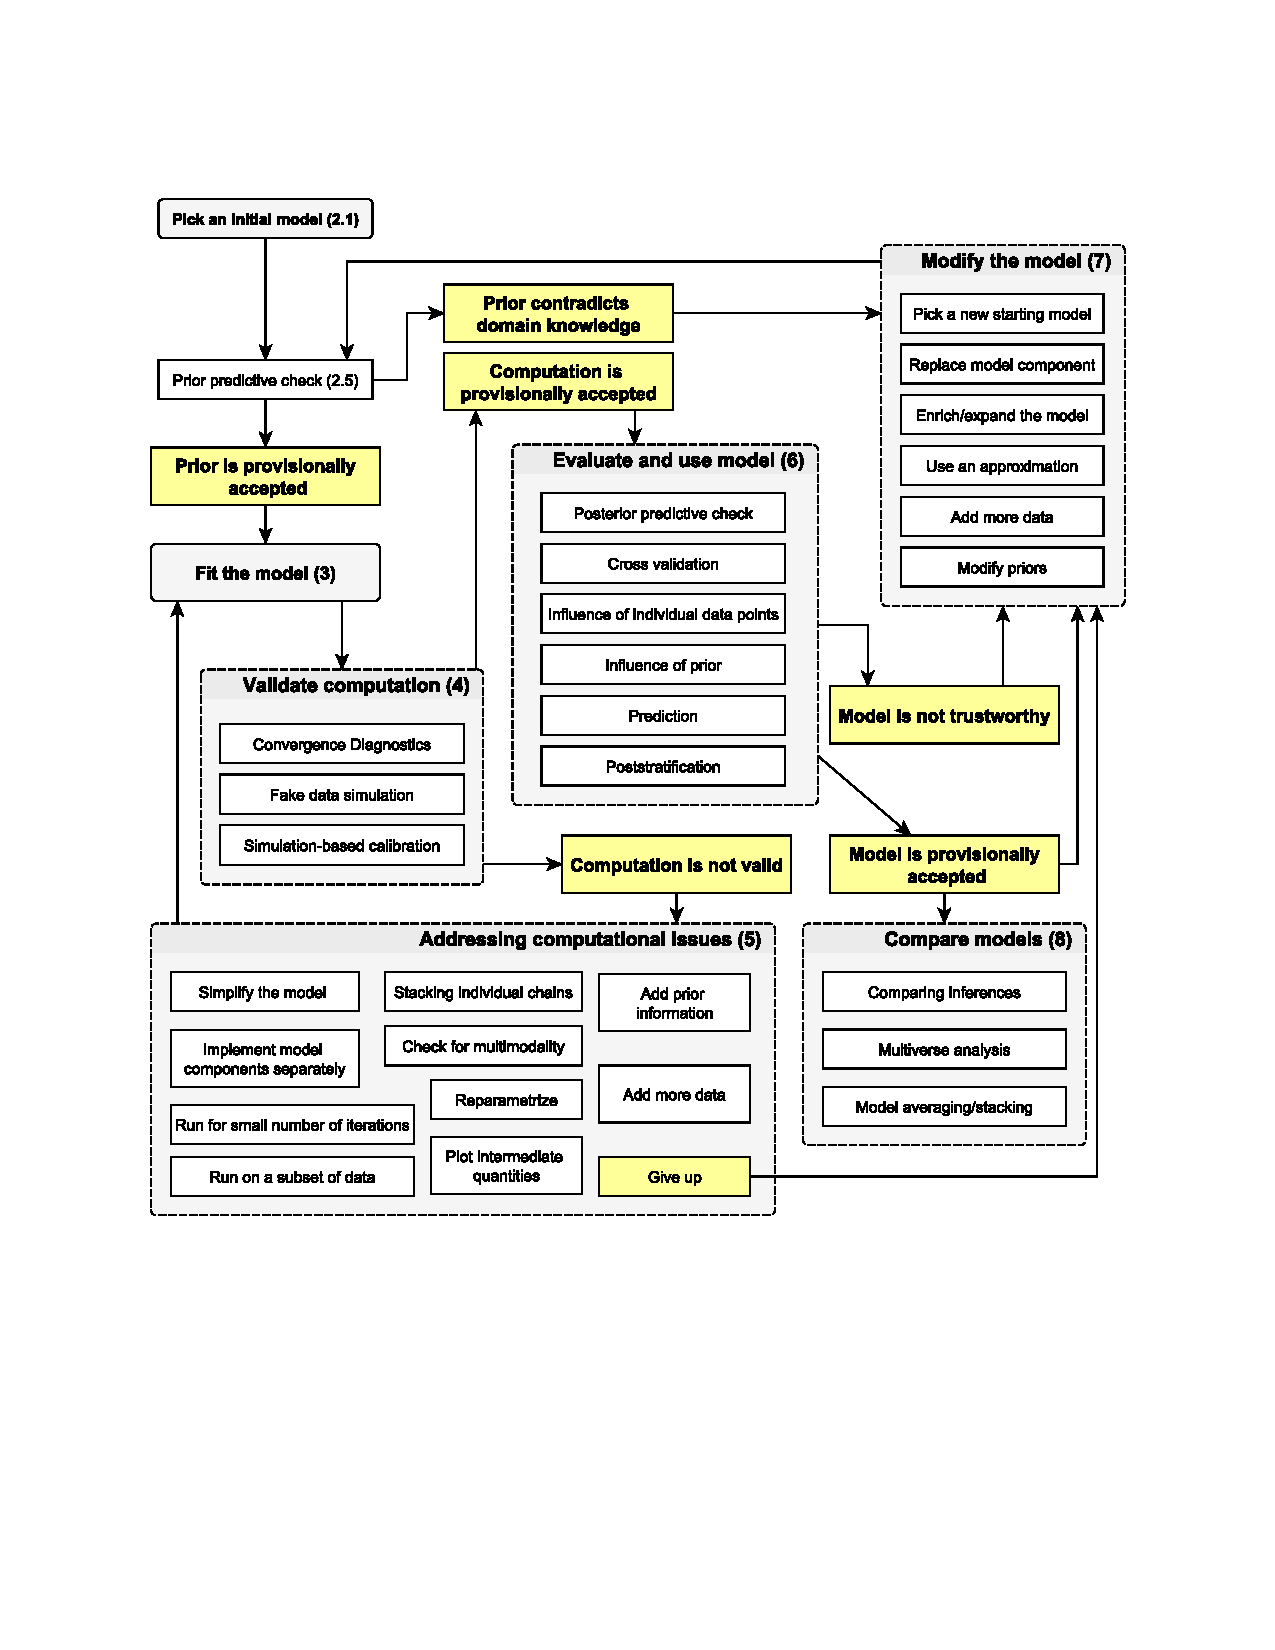
\includegraphics[height=0.7\textheight]{img/workflow-fig.pdf}
\end{center}
\begin{itemize}
\item where else might PPLs help? 
\end{itemize}

